\subsubsection{Pengujian Implementasi}

Hasil implementasi SMOTE dan LN-SMOTE diuji dengan menggunakan Random Forest.
Dataset yang digunakan yaitu dataset phoneme, dengan jumlah atribut 5 dan
dua kelas yaitu $ 0 $ dan $ 1 $.
Jumlah sampel mayoritas, dengan kelas 0, yaitu 3818 sampel dan minoritas
sebanyak 1586, dengan total 5404 sampel.

Dataset di-\textit{resampling} dengan rasio $ 100\% $.
Hasil \textit{resampling} SMOTE menghasilkan 1586 sampel sintetis sehingga
jumlah total semua kelas minoritas menjadi 3172 sampel ($ 45.3\% $ minoritas).
Hasil \textit{resampling} LN-SMOTE menghasilkan 1562 sampel sintetis sehingga
jumlah total semua kelas minoritas menjadi 3148 sampel ($ 45.1\% $ minoritas).

Random Forest diaplikasikan dengan nilai attribut yang dipilih secara acak
yaitu 3, jumlah persentase bootstrap $ 66\% $, dengan nilai \textit{nearest
neighbourhood} 5 dan jumlah pohon sebanyak 50.
Hasil dari klasifikasi \textit{Random Forest} diplot berdasarkan laju galat OOB
untuk setiap hasil \textit{resampling}, seperti yang terlihat pada gambar
\ref{fig:rf_with_resampling_phoneme}.

\begin{figure}[t]
	\centering
	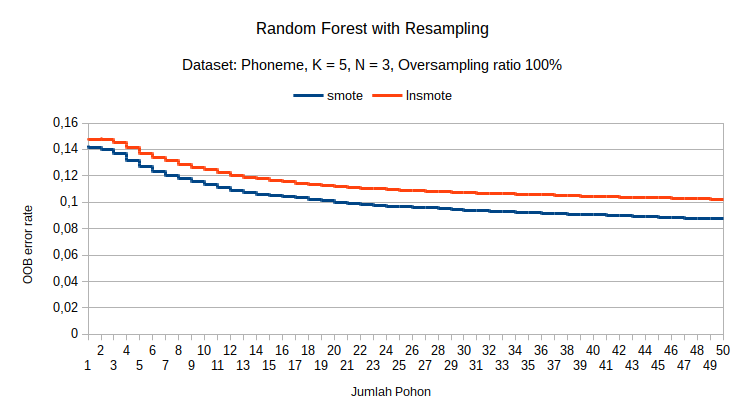
\includegraphics[keepaspectratio=true,scale=0.7]{rf_with_resampling_phoneme}
	\caption{Hasil uji \textit{resampling} dengan pengklasifikasi \textit{Random Forest}}
	\label{fig:rf_with_resampling_phoneme}
\end{figure}
